\chapter{Results} 
\section{Overview}

Neural Network architecture plays a significant role in the performance of a NN. The training period requires a balance between the incorporation of new information, learning and retention of old information, memory. Various architectures train themselves in a variety of ways and thus process training data very differently. Additionally, inputs fed into a NN as well as the quality of the training set can greatly impact its efficacy in making accurate predictions. \textbf{Table \ref{table:overall_performance}} shows the performance of each program from each article.

\begin{table}[h!]
    \centering
    \includegraphics[width=0.6\linewidth]{./images/overall_performance.png}
    \caption{\textbf{Performance of each NN within the selected literature.} Different metrics selected to indicate performance over multiple test sets makes analysis fairly difficult.}
    \label{table:overall_performance}
\end{table}

\subsection{Residual Neural Networks}

Many of the selected literature provided programs that utilised a residual network (ResNet) architecture \cite{seniorImprovedProteinStructure2020,xuAnalysisDistancebasedProtein2019,ruffoloGeometricPotentialsDeep2020,hiranumaImprovedProteinStructure2021,houMULTICOMProteinStructure2020a, liberisParapredAntibodyParatope2018} in some part of the program's structure. This is most likely due to ResNet's ability to apply a deeper neural network without reducing prediction accuracy, whilst still maintaining convolutional layers for automatic feature extraction. 

\textbf{\subsubsection{RaptorX \cite{xuAnalysisDistancebasedProtein2019}}}

RaptorX uses a very deep ResNet to predict the Pythagorean distances between pairs C\textsubscript{$\beta$} atoms from two distinct residues. The NN at its core aims to predict distances between C\textsubscript{$\beta$} of pairs of residues. A multiple sequence alignment (MSA) is produced using homologous proteins, which provides co-evolutional data. Residues that mutate together in a similar time frame indicate close proximity in space. The creators of RaptorX employed two separate ResNets, one that accepts 2D matrix inputs, and another that accepts 3D matrices, utilising 7 and 60 convolutional layers respectively. Distances between C\textsubscript{$\beta$} are placed into separate categories for classification. The system was trained using 11,410 non-redundant proteins, with 900 forming the validation set.

\textbf{\subsubsection{AlphaFold \cite{seniorImprovedProteinStructure2020}}}

At its core AlphaFold has a deep two-dimensional residual network. The fundamentals that form this residual network originate from the RaptorX predecessor \cite{wangAccurateNovoPrediction2017}, thus there are many structural similarities. 
\\[12pt]
Similar to RaptorX, AlphaFold organises spatial distances into discrete categories for classification and whilst the network architectures vary, they receive similar inputs such as co-evolutional MSA inputs and secondary structure. The heart of the inter-residue distance prediction is a deep two-dimensional dilated ResNet. The network is formed of 220 residual layers, with dilated convolutions; which produce dense predictions \cite{yuMultiScaleContextAggregation2016}. AlphaFold is trying to predict inter-residue distance between every residue within the structure, dissimilar from image recognition where an object is being recognised and annotated, thus dilated convolutions are used to provide better prediction capabilities for the given input. The NN's complexity is enabled by the ResNet structure and their vast training set of 31,247 protein domains sourced from the PDB \cite{bermanProteinDataBank2000a}. Furthermore, AlphaFold employ a folding network that aims to fold the proteins by minimising the gradient descent, allowing them to minimise folding error. 


\textbf{\subsubsection{DeepH3 \cite{ruffoloGeometricPotentialsDeep2020}}}

DeepH3 uses a deep residual network of 1D and 2D convolutions, to structurally model the H3 CDR loop. The NN predicts distances between C$_\beta$ on separate residues, by taking samples of pairs within the loop. DeepH3 only utilises the protein sequence with no other data, MSAs etc. and still obtained valuable predictions. Unfortunately DeepH3 only reported the Pearson correlation and circular correlation coefficients (\textbf{Figure \ref{table:overall_performance}}), again making a comparison to other programs difficult. 

\textbf{\subsubsection{DeepAccNet \cite{hiranumaImprovedProteinStructure2021}}}

DeepAccNet taxes inputs of atomic coordinates that are processed in convolution layers. Which is then flattened and passed through a ResNet with 24 layers. The model was trained on 8,718 protein chains, whilst this is a large dataset for a shallow network, the authors did not mention any overfitting prevention techniques or tests. However, a test data set was correctly applied, which mitigates this concern. 

\textbf{\subsubsection{ParaPred \cite{liberisParapredAntibodyParatope2018}}}

The ParaPred deep learning model utilises an antibody primary sequence, from which it extracts the CDR sequences using the Chothia numbering scheme \cite{al-lazikaniStandardConformationsCanonical1997} with an additional two residues on each side of the CDR as these are known to be involved with binding \cite{krawczykAntibodyIPatchPrediction2013}. It then outputs a prediction for each residue between 1 and 0, depending on whether they are predicted to bind or not bind respectively. This model is composed of a CNN that feeds into a recurrent neural network (RNN), it also includes some ResNet properties, including shortcut connections within the RNN to allow a more complex model. The CNN processes amino acid sequences via a 3D input matrix with each sequence constituting a new row, and the max sequence length setting the number of columns (\textbf{Figure \ref{fig:ParaPredMatrix}}), on the z-axis there are 21 layers that account for 20 amino acid types + 1 unknown type. A binary 1 or 0 in any of these slots will represent what amino acid is in the respective cell. 

\begin{figure}
    \centering
    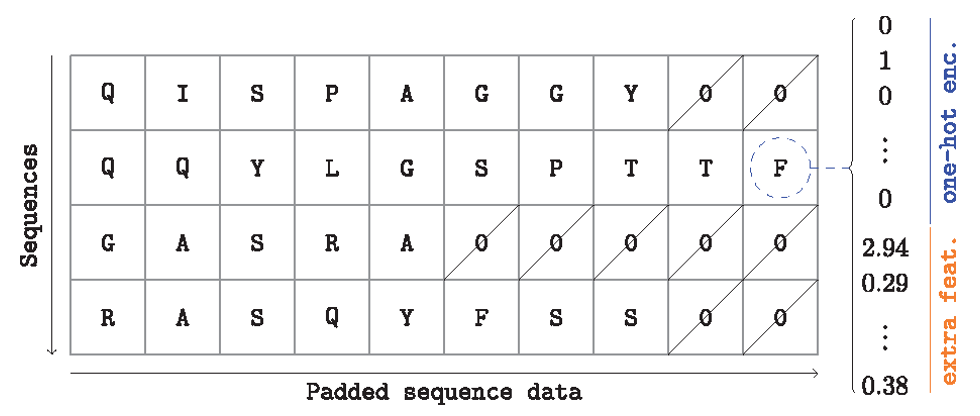
\includegraphics[width=\linewidth]{./images/parapredsequence.png}
    \caption{\textbf{ParaPred CNN input matrix.} Taken from ParaPred's article \cite{liberisParapredAntibodyParatope2018}. Each row represents a new CDR sequence and the max number of columns is set by the longest sequence, with shorter sequences being padded by empty 0 values.}
    \label{fig:ParaPredMatrix}
\end{figure}

\textbf{\subsubsection{Potential Overfit}}
Whilst reviewing the ParaPred paper, one of my initial concerns was the small dataset compiled from the SAbDab \cite{dunbarSAbDabStructuralAntibody2014}, a database of antibody-antigen crystal structures compiled from the protein data bank \cite{bermanProteinDataBank2000a} a larger database of various protein structures. ParaPred's dataset only consisted of 277 antibody-antigen complexes. Additionally, the validation set was used to tune the parameters of the network, and then the NN was evaluated with this validation set instead of a separate test set. The retuning may have introduced a bias, meaning their results are potentially unreliable.
\\[12pt]
I tested ParaPred for an overfit and found no significant difference in prediction error of a test set of three antibody-antigen complexes that ParaPred was trained on and three that the model had never seen. (\textbf{Figure \ref{fig:ParaPredError}}) shows the model's prediction error for each structure, and after performing a Welch t-test found that the difference in means was not significant.
\\[12pt]
ParaPred had not overfitted the data as I originally expected. Whilst this was surprising due to the small data set used to train a complex model, there are a few techniques employed to prevent overfitting. Firstly ParaPred is trained using 10-fold cross-validation; this method trains the model 10 times from scratch with 10 varying test sets and training sets, aiming to highlight if a model is overfit. Additionally, the model is regularized via weight decay and dropout \cite{srivastavaDropoutSimpleWay2014a}. On each training loop of the RNN, random inputs are removed from neurons in the network, to prevent the model relying on one particular set of inputs. Weight decay targets parameters that have grown too large during training and reduces their effect, essentially preventing aggressive output influence from small areas of the network. These factors combined, cleverly helped negotiate the issue of overfitting in creating a complex model that was trained using such a small dataset.


\begin{figure}
    \begin{small}
        \begin{center}
            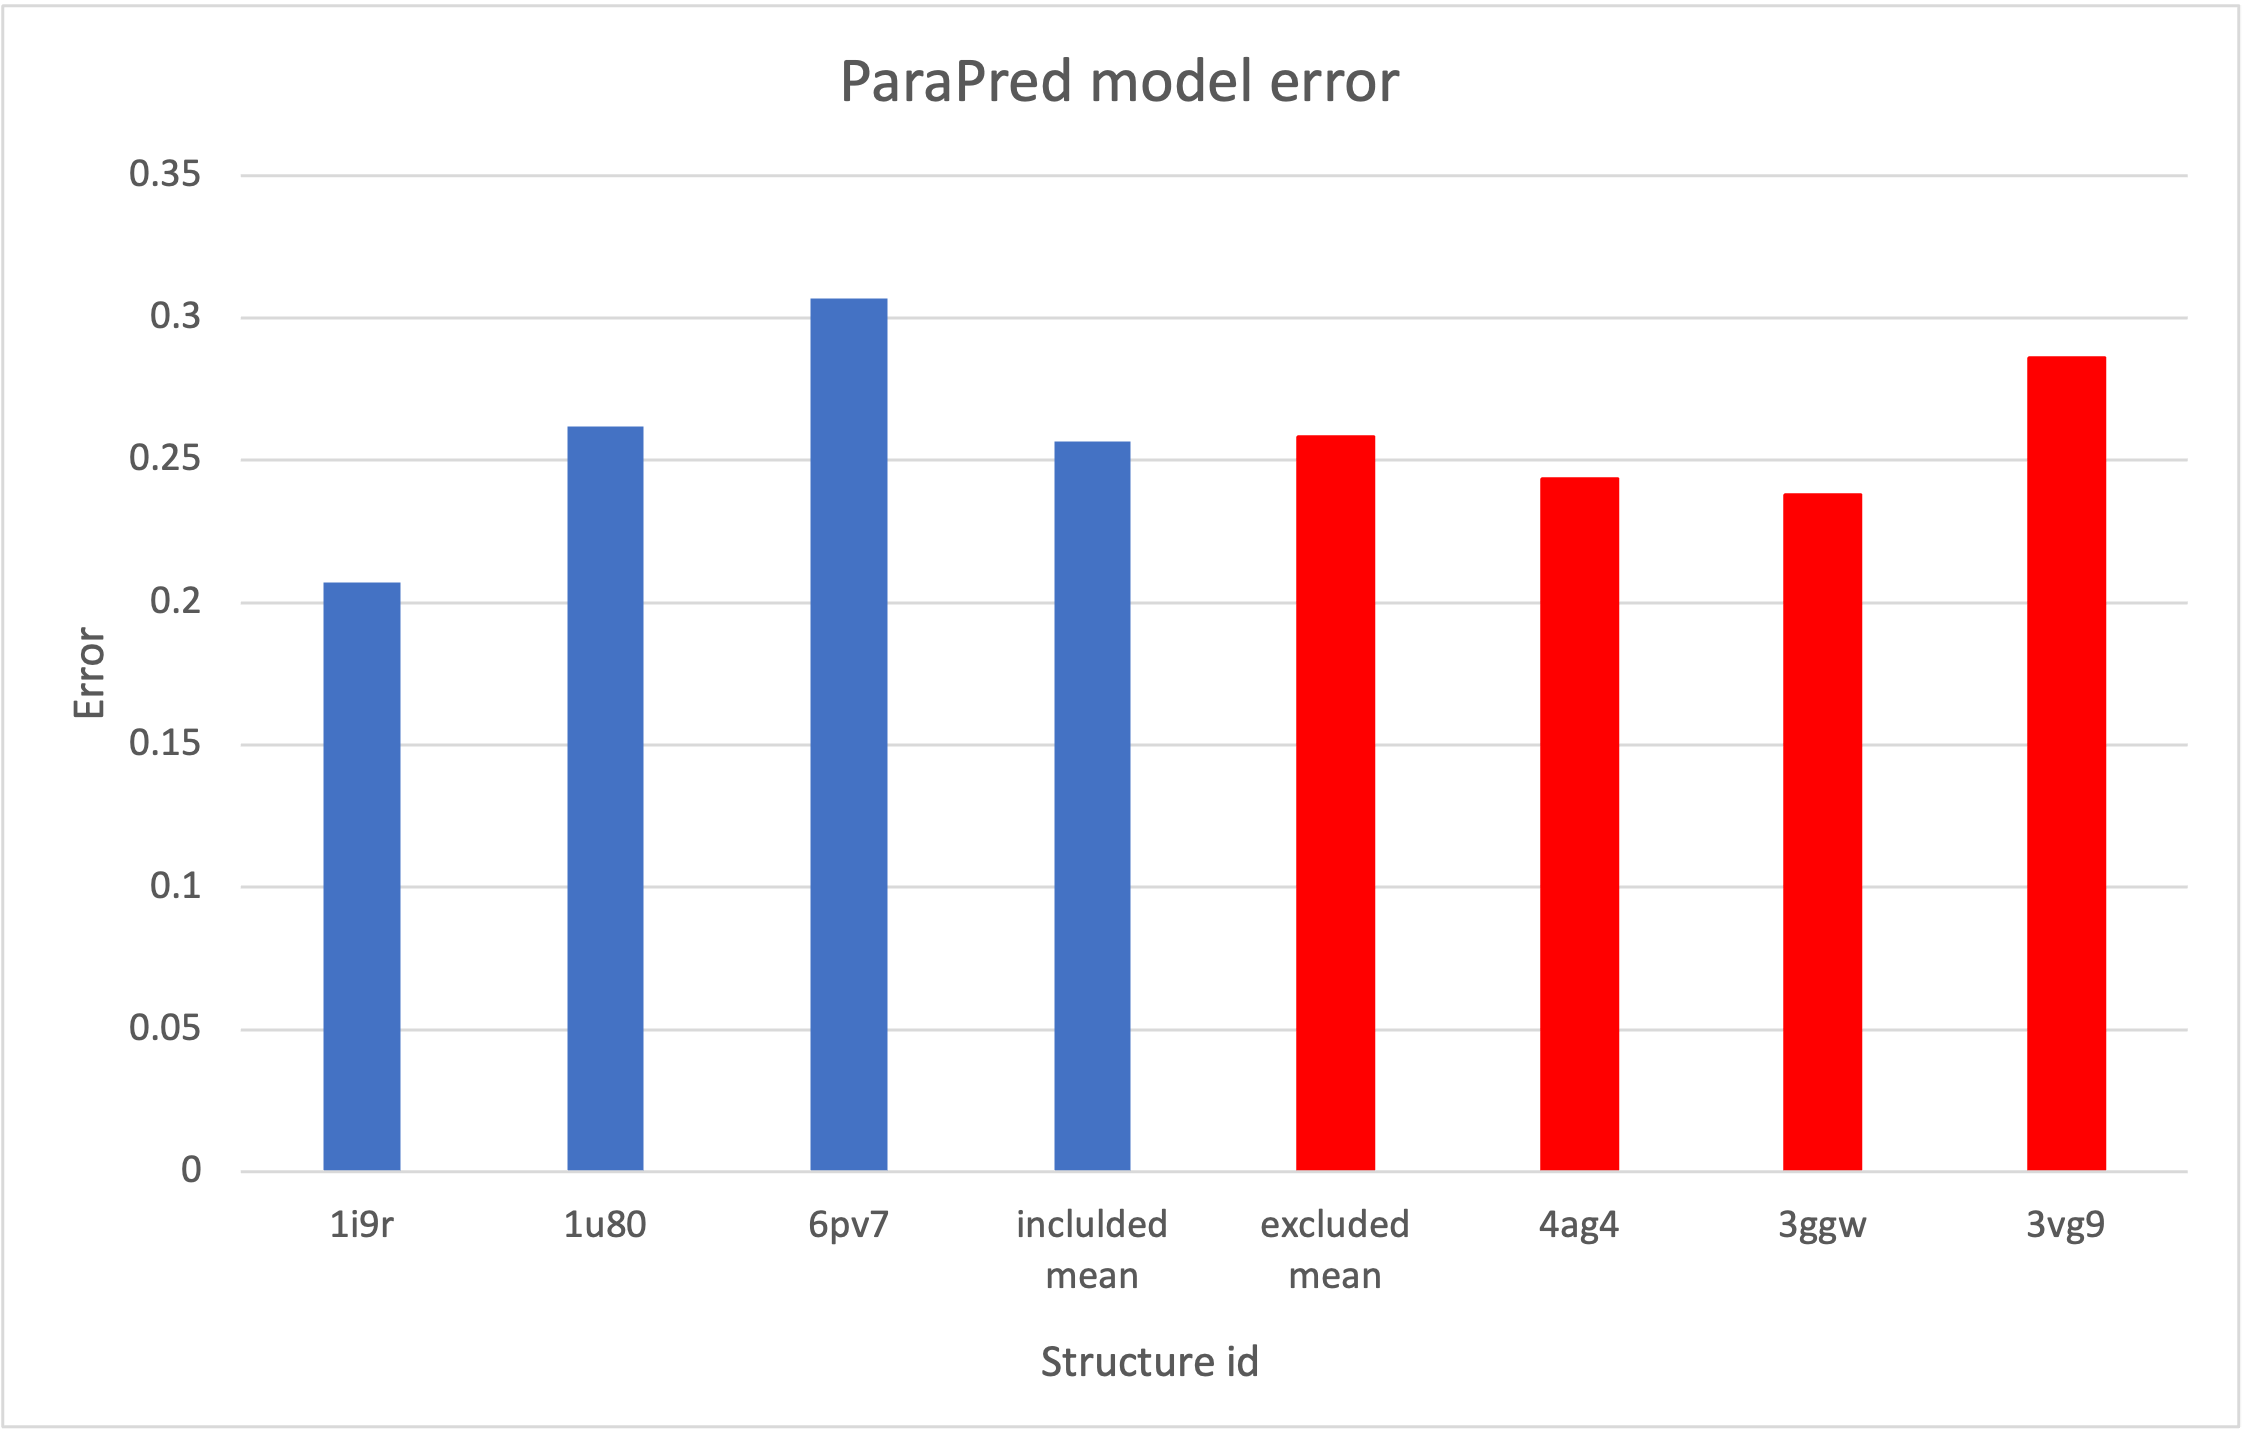
\includegraphics[width=0.95\textwidth]{./images/parapred_error.png}
        \end{center}
        \caption{\textbf{ParaPred overfitting test results.} Three blue bars represent structures 1i9r, 1u80, 6pv7 (PDB ids) that were not part of the training set. Three red bars represent structures 4ag4, 3ggw, 3vg (PDB ids) that were part of ParaPred's training set. Mean of the errors shown as the two centre bars. }
        \label{fig:ParaPredError}
    \end{small}
\end{figure}


\subsection{Convolutional Neural Networks}

NNs that were created with a CNN architecture were limited in depth and complexity, but in many cases this was to prevent overfitting specifically in the interaction prediction literature \cite{balciDeepInterfaceProteinproteinInterface2019}, due to the lack of antigen-antibody complexes available for use as training data. ParaPred \cite{liberisParapredAntibodyParatope2018} utilised a CNN to analyse local interactions between 

\textbf{\subsubsection{DeepInterface \cite{balciDeepInterfaceProteinproteinInterface2019}}}

DeepInterface aims to classify proteins that are in a docked state and determine whether or not that is a natural bound conformation. Protein structures that are to be inputted to the model are presented as voxels, a voxel to a 3D structure is essentially what a pixel is to an image, it represents a point in 3D space. Protein complexes were collected from a variety of sources, and to ensure that there were some proteins that were not bound with the correct residues contacting the authors used an algorithm named ZDOCK. This is a vital step, as without these 'negative' structures, the NN would not be able to differentiate between correctly bound and incorrectly bound structures. DeepInterface was trained on an enormous 271,830 separate interfaces, for such a shallow network this training set is incredibly large and hints at why the NN's performance exceeded expectations, achieving 75\% accuracy on a test dataset. However, there was a possible overfit as the model did achieve a better accuracy of 92\% and 88\% in the training and validation sets respectively.

\textbf{\subsubsection{DNN-PPI \cite{liDeepNeuralNetwork2018}}}

DNN-PPI utilised primary protein sequence without any additional information, the sequence was passed into a CNN and then to a long short-term memory NN. Over 70,000 structures were extracted for training with ~8000 being used as a validation set (N.B. in the article the authors mislabel this as a testing set, but the testing set is the mus musculus structures). There are an additional 22,870 structures used as a test set. Additionally, DNN-PPI implement good techniques to prevent overfitting such as 5-cross fold validation. On the test set DNN-PPI scored a prediction accuracy of 92.43\% which is very high, and likely due to their significant dataset. Additionally, the selection of a LSTM network appears to be an important feature. To maximise the value of the dataset, some features of previously seen inputs must be retained so they can be combined with the current sequence of the data that the model is processing, which the LSTM network is excellent at, likely contributing to the high accuracy of this NN.

\textbf{\subsubsection{DPPI \cite{hashemifarPredictingProteinProtein2018}}}

DPPI, like DeepH3 utilises minimal input data including the primary protein sequence and a PSI-BLAST search. It aims to predict antigen The core architecture is formed of a Siamese-like CNN, which are primed to learn relationships between two entities. Interestingly DPPI is trained using an unsupervised data set, that is unlabelled; this allows the model to train itself without having to source labelled data, but can lead to lower quality predictions. Unlike AlphaFold and RaptorX who use classification techniques using categories for inter-residue distances, DPPI uses a regression model, which can predict a continuous output for residues between the proteins. 10-fold cross validation is employed like that with ParaPred. Even though the NN was tested on 'benchmark' datasets, the model was trained using these datasets with validation sets being used as a make shift test set, with the lack of a true test set; results are likely biased, therefore their high accuracy of 94.55 percent could be unreliable. 

\textbf{\subsubsection{MULTICOM \cite{houMULTICOMProteinStructure2020a}}}

MULTICOM \cite{houProteinTertiaryStructure2019} like other neural networks utilised co-evolution methods, by generating MSAs with homologous proteins and predict secondary structure of the protein sequence which is also fed into the NN. MULTICOM employs a remarkably shallow NN to process all of this information, called DNCON2 described as a separate NN \cite{adhikariDNCON2ImprovedProtein2018}. This CNN utilises 7 convolutional layers for feature extraction in comparison to AlphaFold's 220, and is trained over 1600 epochs in comparison to AlphaFolds 500 epochs, one epoch refers to a single training loop where all training data has passed through the NN. The curators attempted to test up to 9 convolutional layers, but experienced problems caused by overloading the graphics processing unit (GPU) being used to run the NN. No overfitting preventative measures were taken, but overfitting was unlikely to be prevalent on such a shallow network \cite{xuOverfittingRemedySparsifying2019}. Additionally the DNCON2 model was only trained with 1230 proteins from previous CASP assessments.

\textbf{\subsubsection{Point Neural Networks}}

PInet was the only NN to use a PointNet architecture, it utilises pairs of point clouds of two protein structures to predict interfacing regions. After the local features were extracted using the PointNet, global features were extracted by using pooling together local features, this quickly and with comparatively little computation provides a summary of the proteins' surfaces. The authors implemented a data augmentation technique to prevent overfitting while training on small datasets, this was achieved by randomly rotating certain structures in the training data, producing slightly altered duplicates as further training data. Again it was unclear whether the test dataset remained excluded until parameters were tweaked, therefore the results may not be reliable. PInet did achieve a fairly high AUC-ROC score of 0.867, but a low precision of 51.8\%. Whilst this NN was designed for general protein-protein interactions it was trained with a dataset consisting of antibody-antigen complexes, it scored slightly worse in this dataset potentially suggesting antibody-antigen interactions are more complicated. However, this dataset was significantly smaller than the other training datasets, which could have affected the performance instead.

\subsection{Comparison using CASP13 data}

Three out of the five papers relating to protein structure prediction described models that were entered into the 13th Critical Assessment of Protein Structure Prediction (CASP13): AlphaFold, MULTICOM, and RaptorX \cite{seniorProteinStructurePrediction2019,houMULTICOMProteinStructure2020a,xuAnalysisDistancebasedProtein2019}. CASP13 is an independent accessible competition to identify computational programs that produce the best protein structure predictions. The competitors are presented with the amino acid sequences of target proteins, from which they have to determine the proteins tertiary and quaternary structure. Participants submit five of models towards each of the 84 protein structures.
\\[12pt]
CASP13 provides two main categories for assessment: free modelling (FM) and template based modelling (TBM). Structures fall into the TBM category if part of their structure is available on the public domain via a sequence search, meanwhile FM proteins have no identifiable segments available; thus the computational program has to predict the structure without assistance. 
\\[12pt]
Neural networks are ranked by a global distance test total score (GD\_TS). The GDT\_TS provides a more accurate measurement of similarity between two protein structures, in this context, the modelled structure vs experimentally determined structure; allowing the NN accuracies to be determined. It represents a percentage of residue's alpha carbons falling within a certain cut-off distance of the experimentally determined structure, thus a score must be between 0 and 100. CASP13 produces a GDT\_TS average of 4 GDT with different cut-off values of 1,2,4, and 8 Å, forming the final GDT\_TS.

\begin{figure}[H]
    \centering
    \begin{subfigure}{0.5\textwidth}
        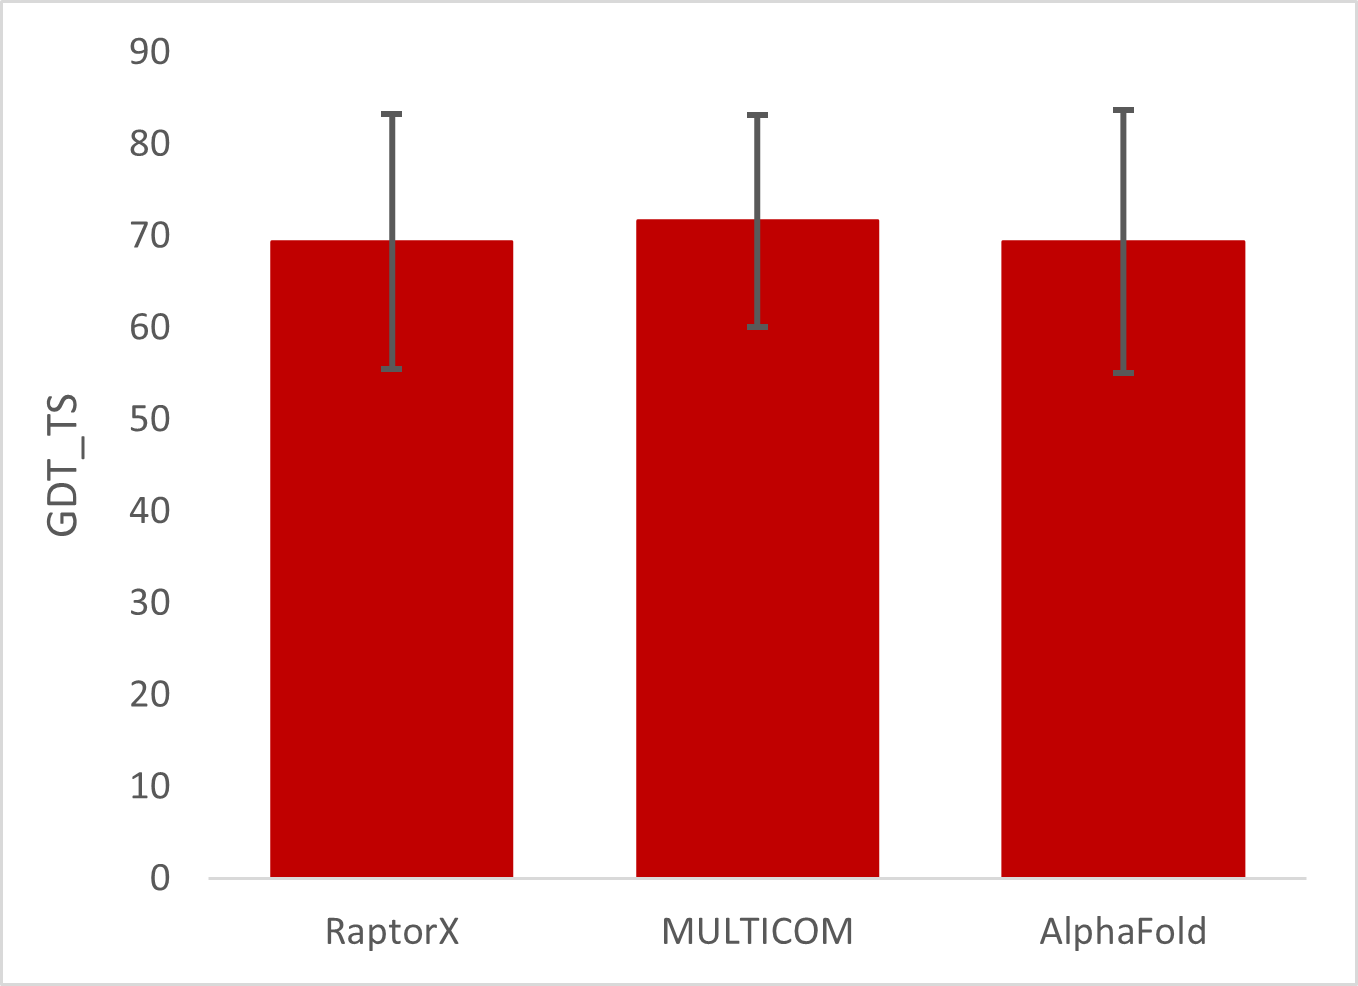
\includegraphics[width=0.8\linewidth]{images/CASP_TBM.png}
        \caption{Template based modelling (TBM)}
        \label{fig:CASP13_TBM}
    \end{subfigure}%
    \begin{subfigure}{0.5\textwidth}
        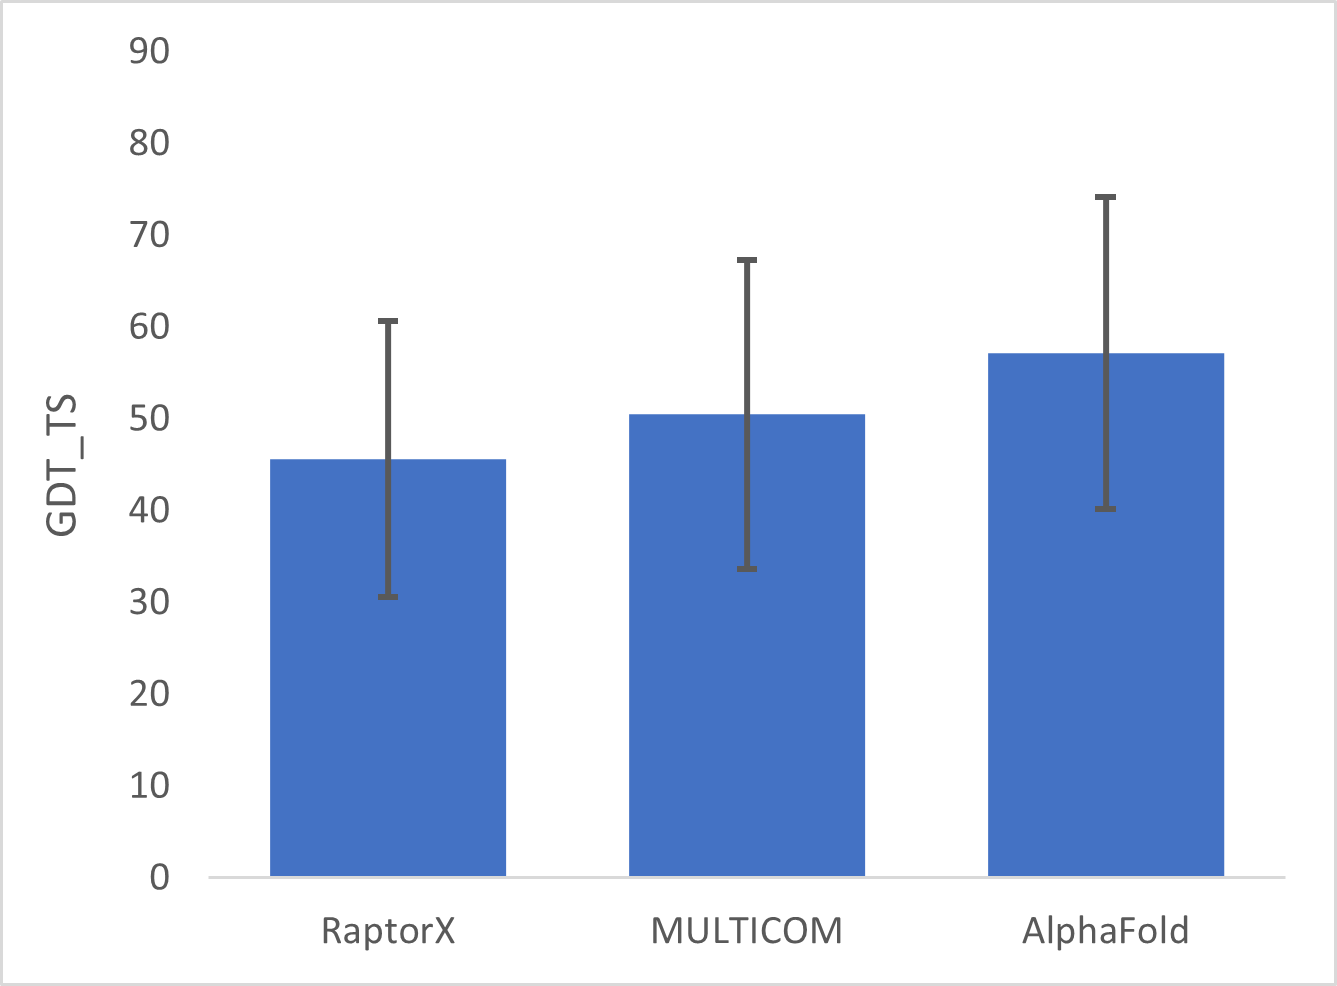
\includegraphics[width=0.8\linewidth]{images/CASP_FM.png}
        \caption{Free modelling (FM)}
        \label{fig:CASP13_FM}
    \end{subfigure}
    \caption{\textbf{Performance of three deep learning neural networks in CASP13.} GDT total score shown on y-axis for a. Template based models, and b. free models. The error bars represent the standard deviation.}
    \label{fig:CASP13}
\end{figure}

\textbf{Figure \ref{fig:CASP13}} shows the data available from the CASP13 website (\href{https://predictioncenter.org/casp13/}{predictioncenter-.org/casp13}). In the template based modelling dataset (\textbf{Figure \ref{fig:CASP13_TBM}}) MULTICOM performs slightly better than both Raptor and AlphaFold, but this does not represent a significant difference. In the free modelling category (\textbf{Figure \ref{fig:CASP13_FM}}) AlphaFold performs significantly better than RaptorX, and slightly better than MULTICOM, but not a significant amount. It is important to note, that whilst RaptorX does not perform as well as MULTICOM and AlphaFold in the results shown here; the model performed significantly better in a separate contact prediction category (\textbf{Figure \ref{fig:CASP_contact}}).
\\[12pt]
Models perform remarkably well in the TBM category and fairly well in the FM category. FM represents a harder but more realistic challenge, as many protein structures are still unsolved. Whilst these seem promising, it is thought that a different metric known as GDT high accuracy (GDT\_HA) performs better in the assessment of structural accuracy producing "more stringent" results, that promote structures useful in drug discovery \cite{readAssessmentCASP7Predictions2007}. GDT\_HA is calculated in the same manner as GDT\_TS, but different cut-off values are incorporated of 0.5, 1, 2, 4 Å, half the distance of the cut-off points used in GDT\_TS.
\begin{figure}[H]
    \begin{small}
        \begin{center}
            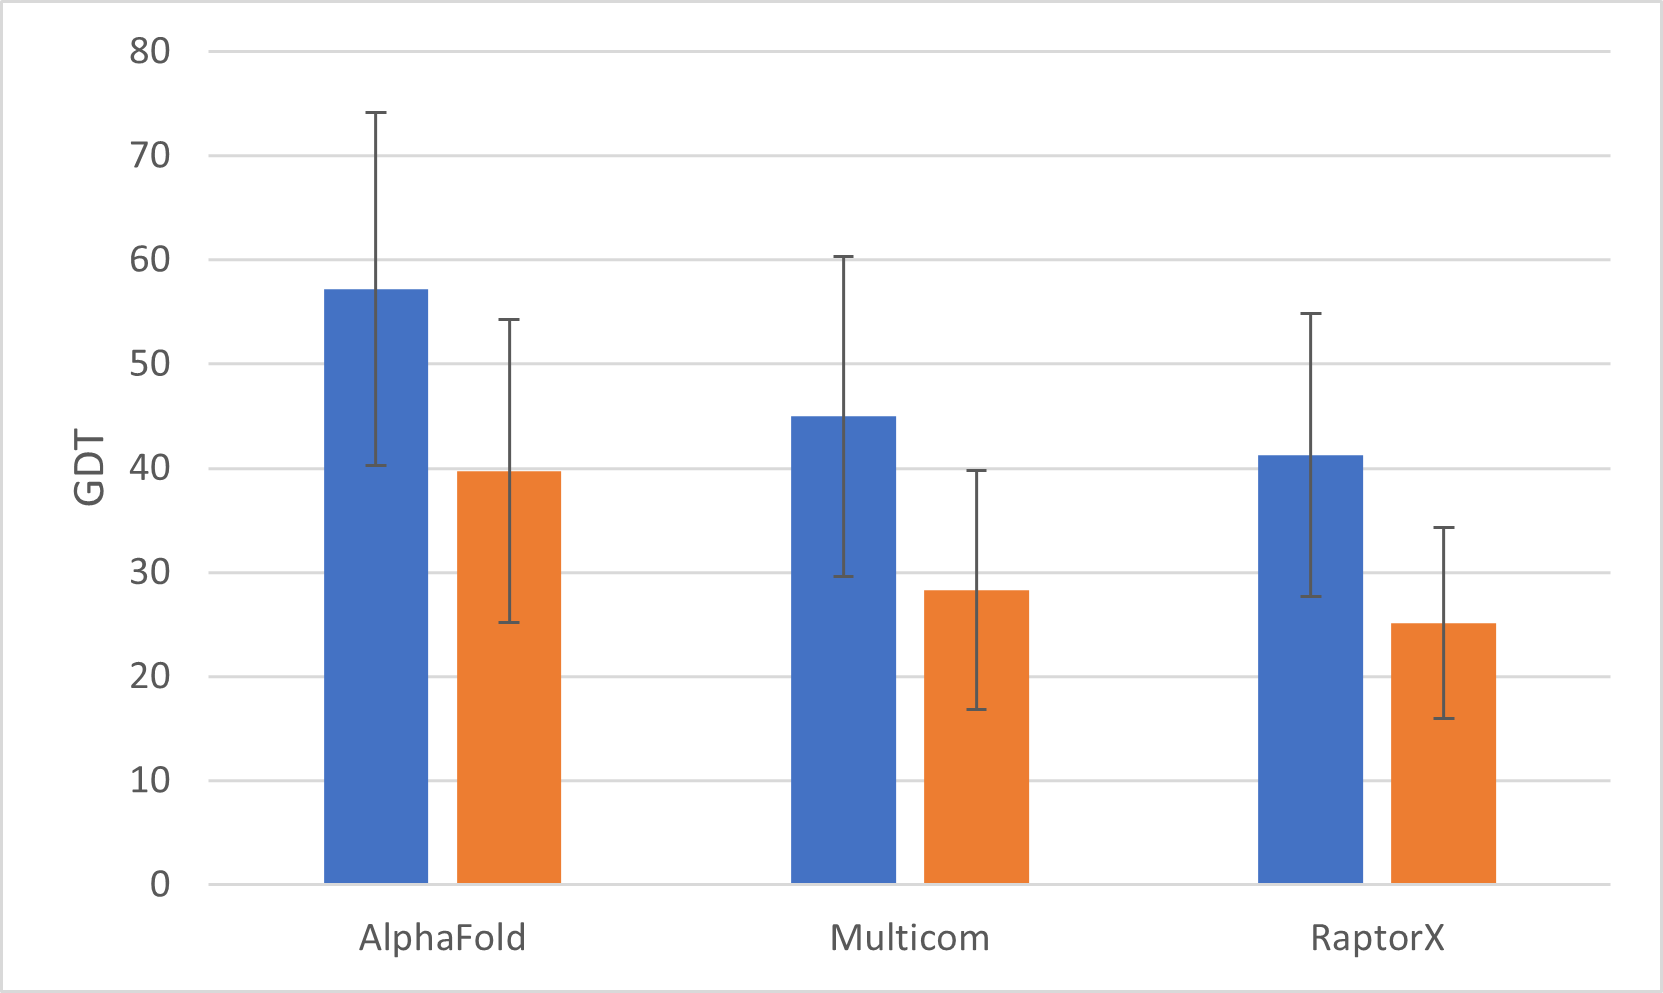
\includegraphics[width=0.95\textwidth]{images/CASP_HA.png}
        \end{center}
        \caption{\textbf{Three analysed deep learning models: AlphaFold, MULTICOM, RaptorX \cite{seniorImprovedProteinStructure2020, houMULTICOMProteinStructure2020a,xuAnalysisDistancebasedProtein2019} performance in CASP13.} Global distance test total score (GDT\_TS) shown in blue (left columns) and GDT high accuracy (GDT\_HA) shown in orange columns (right columns). Error bars represent the standard deviation. }
        \label{fig:CASP_HA}
    \end{small}
\end{figure}
\textbf{Figure \ref{fig:CASP_HA}} shows the free modelling values for GDT\_TS (blue) and GDT\_HA (orange), as expected GDT\_HA values are significantly smaller. Values here show a more accurate representation of the computer model's ability in predicting protein structure.
\\[12pt]
Another category, known as contact prediction involves predicting which residues in a protein are contacting one another; this data is normally incorporated into free modelling programs to provide more data for better identification of possible homologues. In the CASP13 assessment, residues were determined as bound if two C\textsubscript{$\beta$} (or C\textsubscript{$\alpha$} in the case of glycine) atoms were within 8Å of each other. Participants were judged on their Z-score which incorporates the expected and obtained values. \textbf{Figure \ref{fig:CASP_contact}} shows RaptorX's performance compared to MULTICOM and AlphaFold.

\begin{figure}[h!]
    \begin{small}
        \begin{center}
            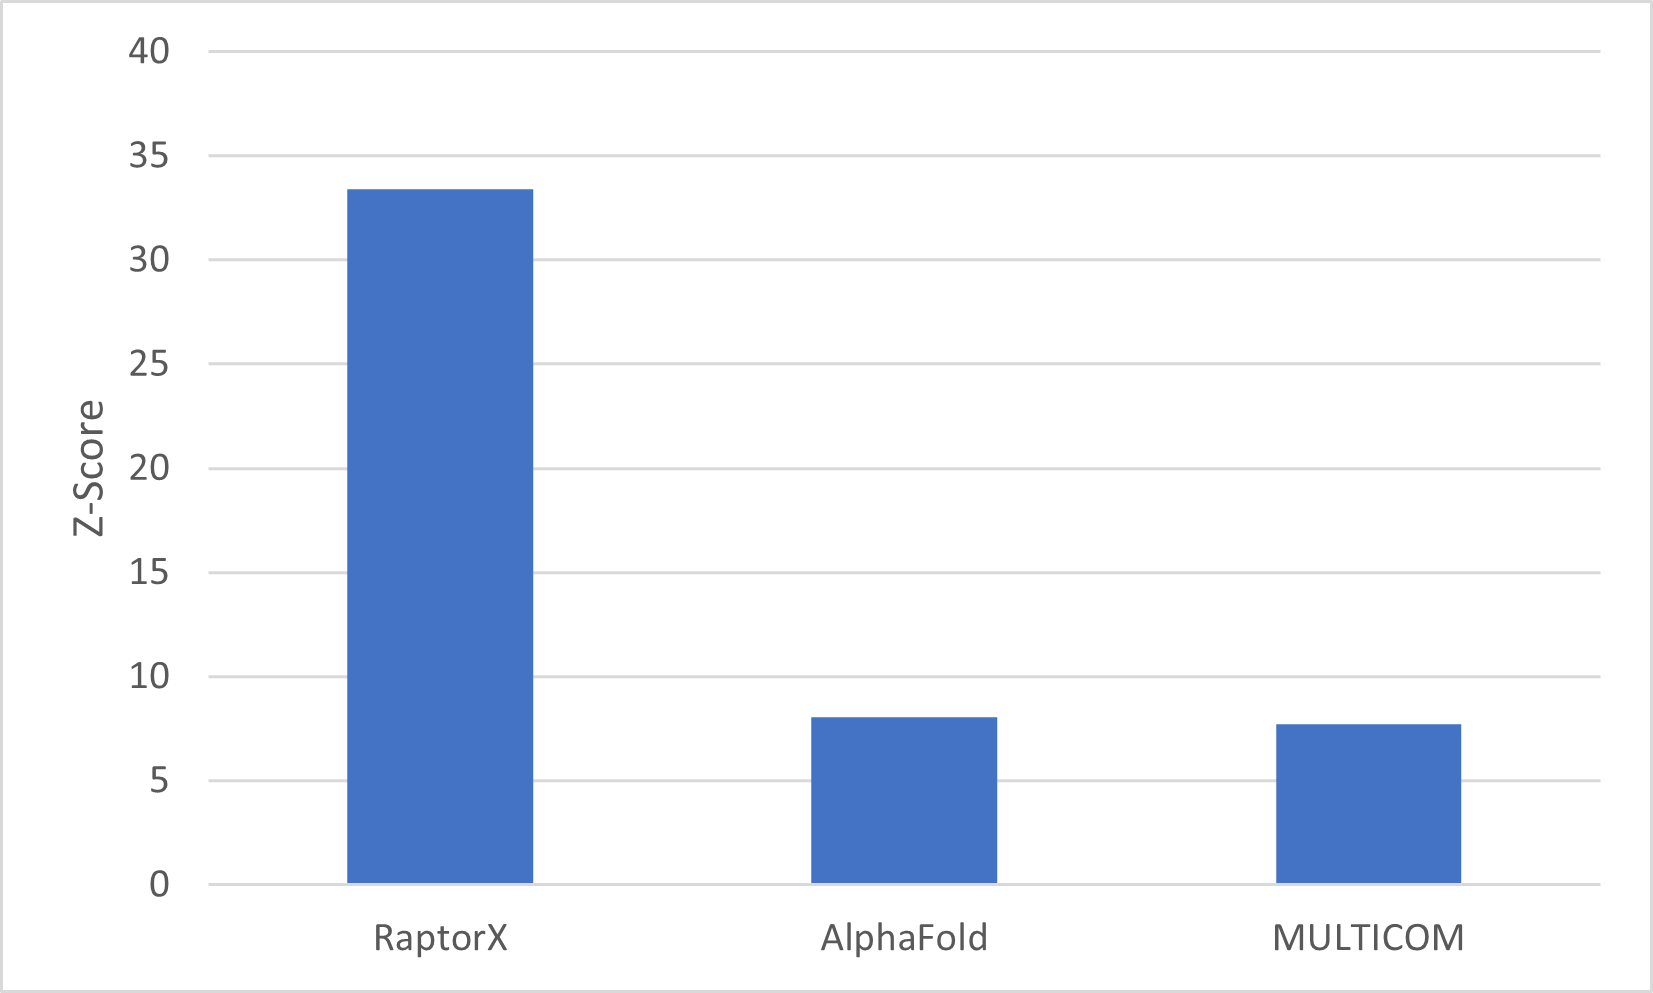
\includegraphics[width=0.95\textwidth]{images/CASP_contact.png}
        \end{center}
        \caption{\textbf{RaptorX, MULTICOM, and AlphaFold performance in CASP13, in the contact prediction category.} Z-score provided for each of the three compared programs.}
        \label{fig:CASP_contact}
    \end{small}
\end{figure}


\subsection{Identifying performance factors} 

My analysis will be focused around the performance in the FM category as this is thought to be the 'harder' of the protein categories to predict, as the computer models are having to predict the full protein structure \emph{ab initio}. 
\\[12pt]
AlphaFold \cite{seniorImprovedProteinStructure2020} performed the best out of the three models, outperforming the nearest competitor by 40\% in the more stringent GDT\_HA assessment. The amino acid sequence is applied using co-evolution methods such as multiple sequence alignments (MSA) with homologous proteins, and residues that mutate together over time are identified. They are likely a result of one residue mutating and the other following to maintain protein structure, thus suggesting a close proximity to one another. It also accepts, protein secondary structure predicted from the SST web server \cite{konagurthuMinimumMessageLength2012}. Results are outputted for every pair of residues in a sequence: distance and psi and phi torsion angles are produced. AlphaFold utilise a very deep 220 block ResNet which is trained over 500 epochs. To prevent overfitting within such a complex network the NN is trained using 31,247 non-redundant protein domains, extracted from the protein data bank (PDB) \cite{bermanProteinDataBank2000a}. Additionally, the creators employed both data augmentation and dropout techniques to reduce the prevalence of overfitting, increasing the viability of such a deep network. Additional, to a complex network, dialated convolutions \cite{yuMultiScaleContextAggregation2016} are used, which can span a larger range than traditional convolution levels, allowing interactions across the whole protein sequence to be analysed.
\\[12pt]
MULTICOM has come under criticism from other teams \cite{xuAnalysisDistancebasedProtein2019}, due to their unclear methodology and surprising performance considering the shallow network utilised. Whilst it is speculative, suggestions were made that MULTICOM "heavily relied on consensus analysis" \cite{xuAnalysisDistancebasedProtein2019} rather than producing a high performance neural network. Potentially providing an explanation for the surprising performance of such a shallow network.
\\[12pt]
RaptorX \cite{xuAnalysisDistancebasedProtein2019} initially process input features with a 1D ResNet, with a depth of 7 convolutional layers. They produce a MSA using HHBlits like that utilised by AlphaFold and MULTICOM  \cite{remmertHHblitsLightningfastIterative2012}, additional inputs include sequence profile, secondary structure, and solvent accessibility. The overall network consists of the 1D ResNet of 7 layers and a 2D ResNet of 60 convolutional layers trained with 10,000 proteins from the PDB. RaptorX massively outcompetes both AlphaFold and MULTICOM in the contact prediction category (\textbf{Figure \ref{fig:CASP_contact}}), but performed significantly worse than AlphaFold in the FM category; potentially indicating a deficiency in their protein folding methodology when compared to AlphaFold.





\subsection{AlphaFold2}

CASP14 took place at the beginning of 2020, and the articles have not yet been released for many of the models or the results; but a notable mention is the successor to AlphaFold, AlphaFold2 \cite{jumperHighAccuracyProtein2021}. AlphaFold performed significantly better in the free modelling category with both GDT\_TS and GDT\_HA scores. Whilst the article is not yet available for review, there is a blog post available providing some detail on how the team achieved such a result (\href{https://deepmind.com/blog/article/alphafold-a-solution-to-a-50-year-old-grand-challenge-in-biology}{https://deepmind.com/blog}). This progress is inspiring, and shows how rapid the advancements in deep learning are. 

\begin{figure}
    \begin{small}
        \begin{center}
            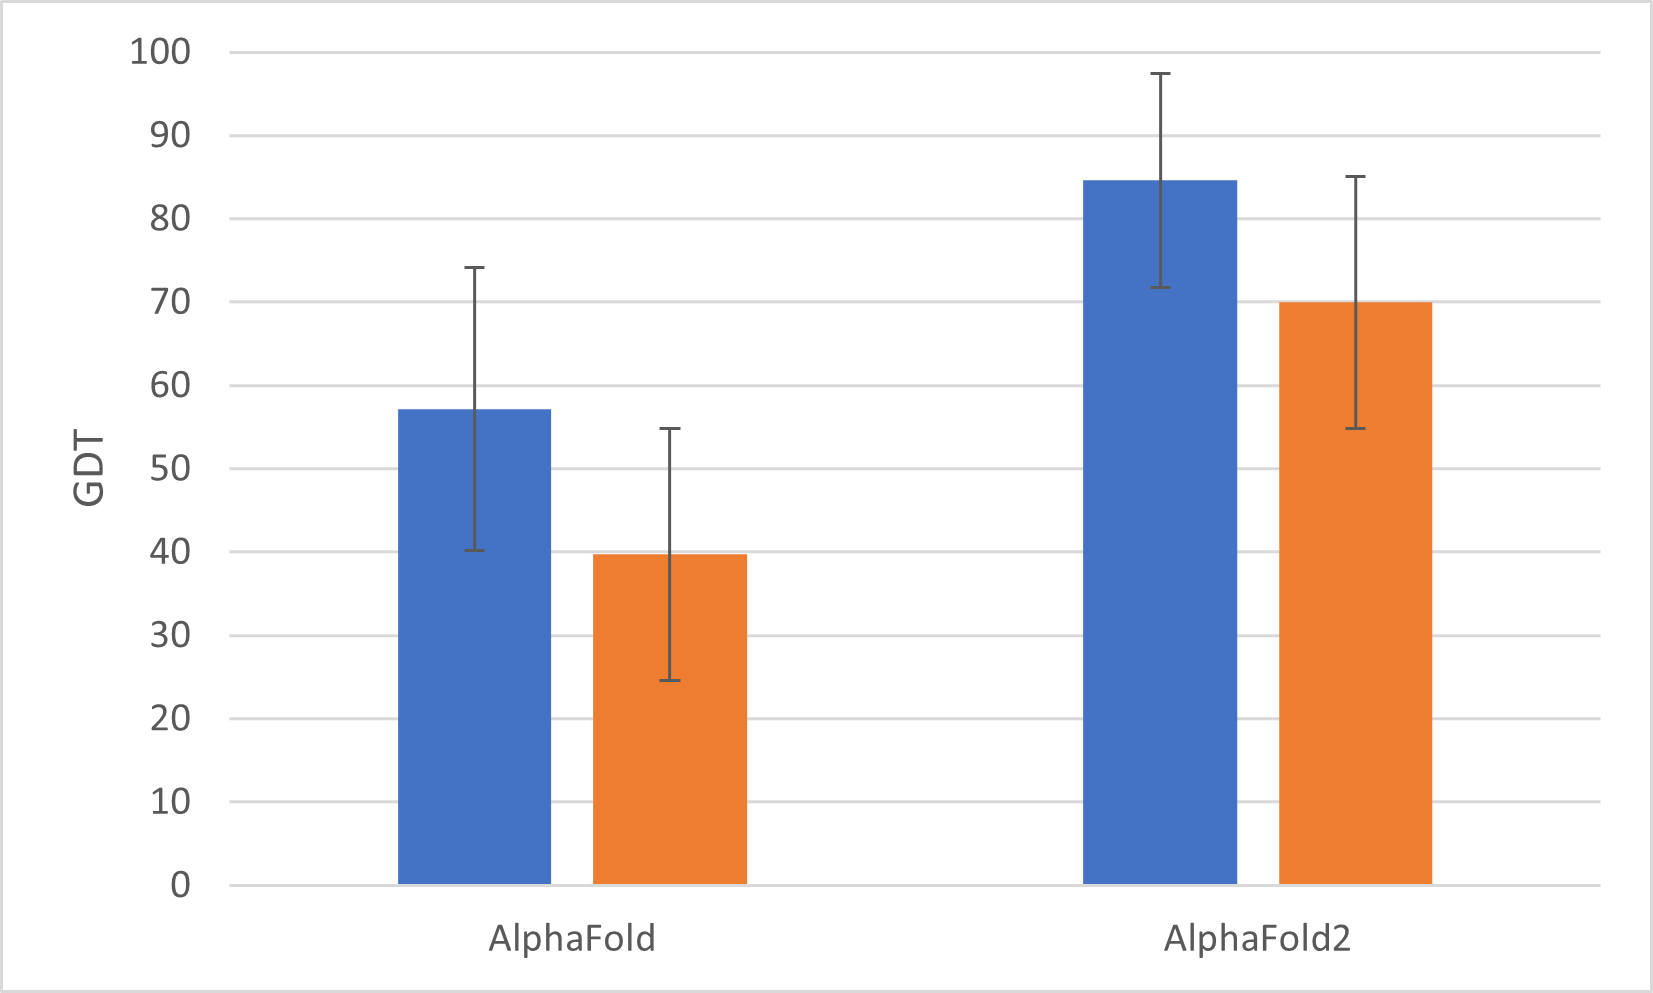
\includegraphics[width=0.95\textwidth]{images/alphafold_comparison.png}
        \end{center}
        \caption{\textbf{Comparison between AlphaFold \cite{seniorImprovedProteinStructure2020} and AlphaFold 2 entered into CASP14.} Blue columns represents GDT\_TS and orange columns denote GDT\_HA scores. Standard deviation is represented by error bars.}
        \label{fig:alphafold_comparison}
    \end{small}
\end{figure}




